%%%%%%%%%%%%%%%%%%%%%%%%%%%%%%%%%%%%%%%%%%%%%%%%%%%%%%%%%%%%%%%%%%%%
%                            Section 5.2
%%%%%%%%%%%%%%%%%%%%%%%%%%%%%%%%%%%%%%%%%%%%%%%%%%%%%%%%%%%%%%%%%%%%
\chapter{5.2 Systems of Linear Equations in 3 Variables}
%%%%%%%%%%%%%%% SECTION HEADER %%%%%%%%%%%%%%%%
\rhead{2}
\lhead{Systems of Linear Equations in 3 Variables}
%%%%%%%%%%%%%%%%%%% START %%%$%%%%%%%%%%%%%%%%%
\section{Introduction}
Solving systems of equations with three variables is very similar to how we solve systems with two variables. When we had two variables, we reduced the system down to one with only one variable (by substitution or addition).\\
In a system with two variables, each equation represent a line in $xy$-plane. If the lines intersect each other, we had \textit{one unique solution}. However, when they don't hit each other, the system have \textit{no solution}. There were also one more possibility: two lines were actually the same line and hit each other at many points. Thus, in this case we had \textit{infinite solutions}.\\
Similar story occurs in a system with three variables. Since we have three variables, $x$, $y$ and $z$, each equation represent a plane in $xyz$-space. There are three possibilities:
%
\begin{itemize}
	\item All three planes intersect each other at exactly one point. We will have one unique solution.
	\item All three planes are parallel and not hitting each other. In this case, we have no solution.
	\item All three planes might intersect at one or more lines or some of the planes might be coincident (same plane). In this case, we have infinite solution.  
\end{itemize}
%
% These possibilities are shown in Figure \ref{fig:planes}.
\begin{figure}[H]
 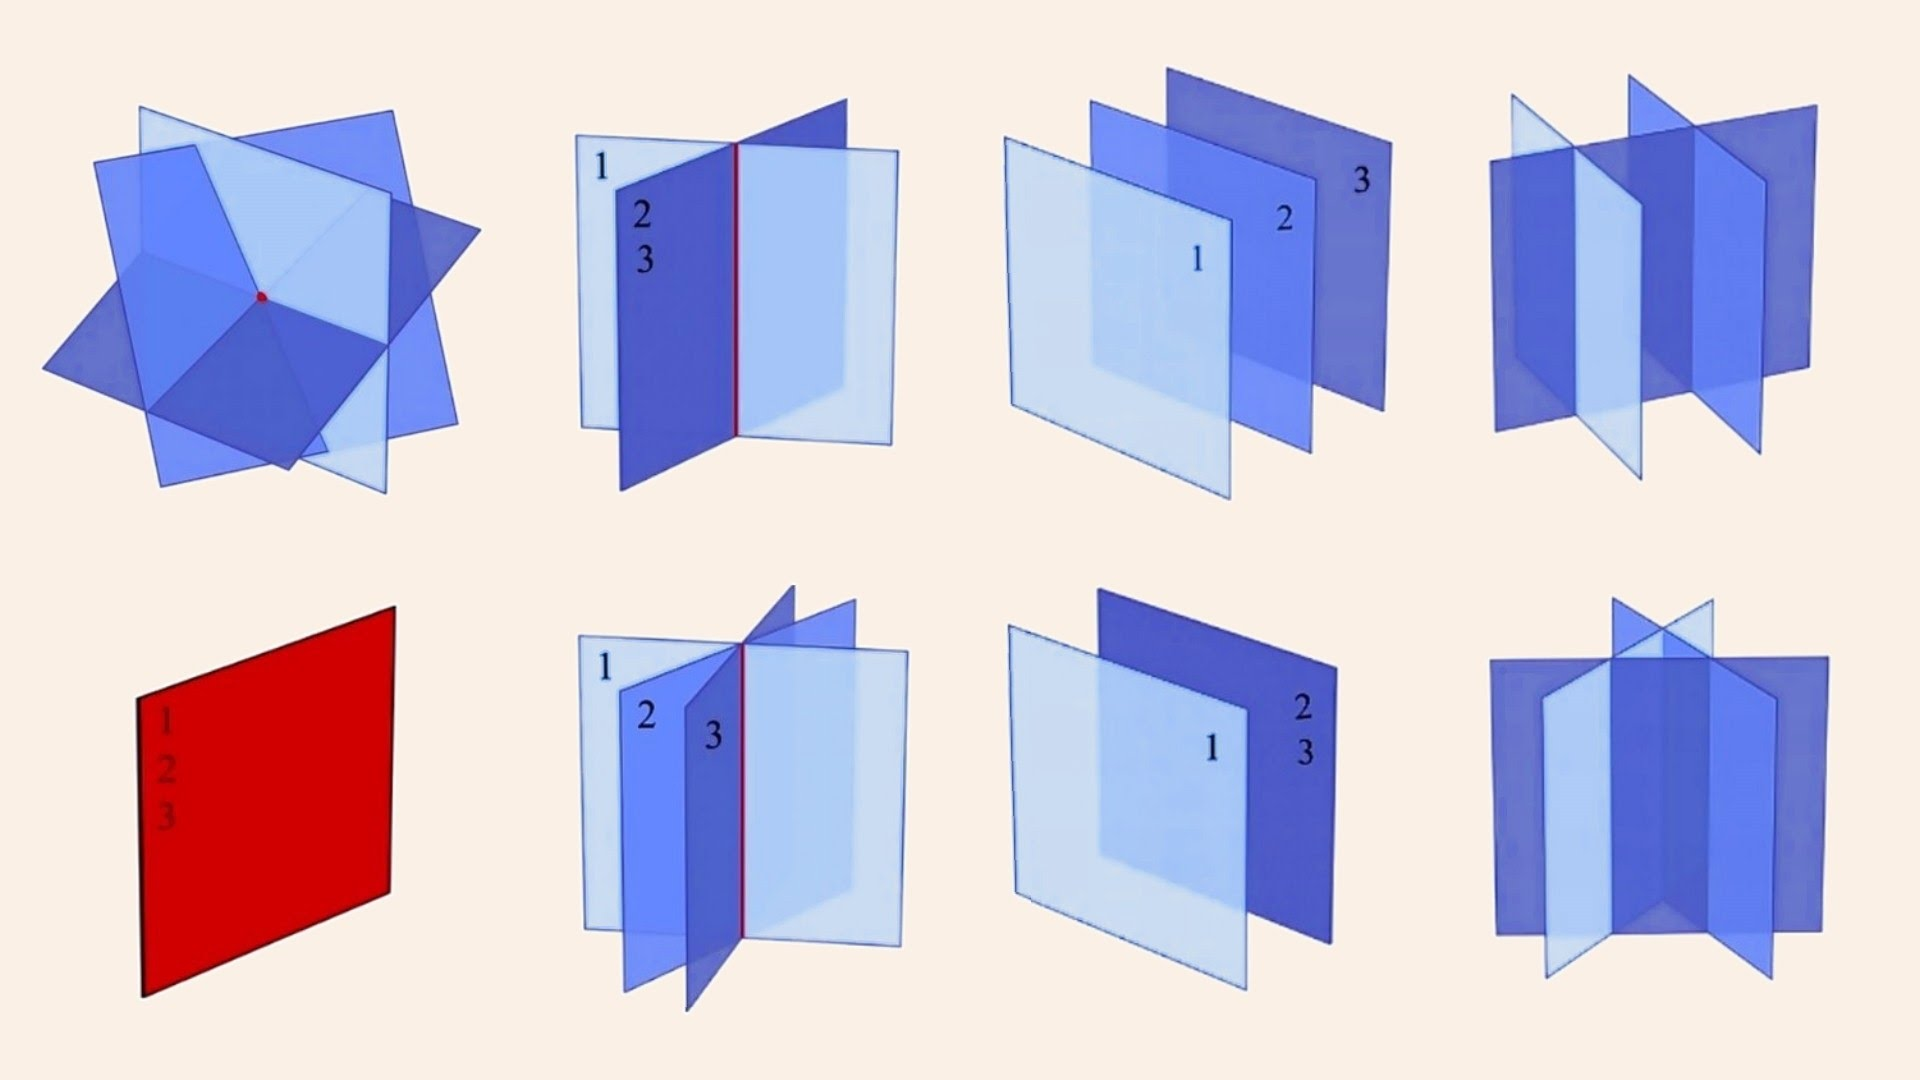
\includegraphics[width=6cm]{pics/planes.jpg}
 \centering
  \caption{Intersection of three planes: all possibilities}
  \label{fig:planes}
\end{figure}
% ======== SECTION
\section{Solving systems with 3 variables}
With three variables we will reduce the system down to one with two variables (usually by addition), which we can then be solved by either addition or substitution. To reduce from three variables down to two it is very important to keep the work organized. 
\vspace{0.5cm}

%
	\begin{tcolorbox}[title=Solve a system with three variables, 
	                  fonttitle=\bfseries,
	                  colframe=blue!70!black,
	                  colback=white]
	\begin{enumerate}
	    \item Choose one variable you want to eliminate. This is entirely up to you.
	    \item Choose two equations and use addition to eliminate the chosen variable. We will call this new equations (A). 
    	\item Then we will use a different pair of equations and use addition to eliminate the same variable. We will call this second new equation (B). 
	    \item We will have two equations (A) and (B) with the same two variables that we can be solved using either method. 
	    \item Find one variable, substitute back into either (A) or (B) to find the other unknown. Then substitute all variables you found in one of the original equations, to find the last unknown.
	\end{enumerate}
	\end{tcolorbox}
%
\vspace{.5cm}


\begin{note}
	In systems with two variables, we had an ordered pair $(x,y)$. In three variables, however, we have an ordered triplet $(x,y,z)$ which represent a point in $xyz$-space
\end{note}
\vspace{.3cm}
%
%============= EXAMPLE 1
\begin{example}
	Solve the system of equations.
		\begin{align*}
		\begin{cases}
			3x+2y-z=-1\\
			-2x-2y+3z=5\\
			5x+2y-z=3
		\end{cases}
	\end{align*}
\end{example}
%
\vspace{0.6cm}

As a first step, Let's eliminate $y$ using two different pairs of equations. Using the first two equations
\begin{empheq}[left={\empheqlbrace}]{align*}
		&x+2y-z     =-1\\
		&-2x-2y+3z  =5
\end{empheq}
%
Notice the coefficients of $y$'s are opposite of each other. So we don't need to multiply either equation by a number. So add them:
%
\begin{align*}
		3x+2y-z&=-1 &&\\
	    -2x-2y+3z&=5 &&\\[-.2cm]
		\cline{1-2}
		x+2z&=4 && \text{Equation (A)}
\end{align*}
%
Using the second two equations, we can find the equation (B). The coefficients of both $y$s are opposite, so just add them to remove $y$
%
\begin{align*}
		-2x-2y+3z&=5 &&\\
		5x+2y-z&=3 &&\\[-.2cm]
		\cline{1-2}
		3x+2z&=8 && \text{Equation (B)}
\end{align*}
Using equation (A) and (B), we can find x and z. We will solve by using Addition. To remove $z$ multiply (A) by $-1$
\begin{align*}
		-x-2z&=-4 && (A)\\
		3x+2z&=8 &&	(B) \\[-.2cm]
		\cline{1-2}
		2x&=4 &&	\text{Divide both sides by 2}\\
		x&=2 && 
\end{align*}
We now have $x$! Plug this into either (A) or (B). We plug it into (A), and solve the equation for $z$
\begin{align*}
	x+2z &=4 && \text{Plug $x=2$}\\
	2+2z &= 4 && \text{Subtract 2 from both sides}\\
	  2z &= 2 && \text{Divide both sides by 2}\\
	z &=1 &&
\end{align*}
We now have $z$! Plug this and $x$ into any original equation. We use the first equation and solve it for $y$
\begin{align*}
	3x+2y-z &=-1 && \text{Plug $x=2$ and $z=1$}\\
	3(2)+2y-(1) &= -1 && \text{Simplify}\\
	 5+2y &= -1 && \text{Subtract 5 from both sides}\\
	 2y &= -6 && \text{Divide both sides by 2}\\
	y &=-3 &&
\end{align*}
We now have $y$! Therefore, our solution is $(2,-3,1)$
%============= NOTE
\begin{note}
In this above problem, y was easily eliminated using the addition method. However, sometimes we may have to do a bit of work to get a variable to eliminate. Just as with addition of two equations, we may have to multiply equations by something on both sides to get the opposites we want so a variable eliminates. As we do this remember it is important to eliminate the same variable both times using two different pairs of equations.	
\end{note}
%============= example 2
\begin{example}
	Solve the system of equations.
		\begin{align*}
		\begin{cases}
			4x-3y+2z=-29\\
			6x+2y-z=-16\\
			-8x-y+3z=23
		\end{cases}
	\end{align*}
\end{example}
No variable will easily removed. We could choose any variable, so we chose $z$. Using the first two equations
\begin{align*}
		4x-3y+2z&=-29 && 4x-3y+2z=-29 \\
		6x+2y-z&=-16\,\, \text{(multiply by 2)} \rightarrow  && 12x+4y-2z=-32 \\
		&&&		\cline{1-2}
		&&& 16x+y=-61\,\, (A)
\end{align*}
We found equation (A). Now use the second two equations (a different pair of equations)
\begin{align*}
		6x+2y-z&=-16\,\, \text{(multiply by 3)} \rightarrow  && 18x+6y-3z=-48 \\
		-8x-y+3z&=23 && -8x-y+3z=23	\\	
		&&& \cline{1-2}
		&&& 10x+5y=-25\,\, (B)
\end{align*}
Using equation (A) and (B), we can find $x$ and $y$
\begin{align*}
		16x+y&=-61\,\, \text{(multiply by -5)} \rightarrow  && -80x-5y=305 \\
		10x+5y&=-25 && \quad 10x+5y=-25	\\	
		&&& \cline{1-2}
		&&& \qquad -70x=280 \\
		&&& \qquad \qquad x=-4
\end{align*}
We have our $x$! You can plug this into either (A) or (B). We plug this into (A)
\begin{align*}
	16x+y &=-61 && \text{Plug $x=-4$}\\
	16(-4)+y&= -61 && \text{Solve for $y$}\\
	 -64+y &= -61 && \text{Add 64 from both sides}\\
	 y &= 3 &&
\end{align*}
We found $y$! Plug this and $y$ into any original equations to find $z$. We plug it into first equation
\begin{align*}
	4x-3y+2z&=-29 && \text{Plug $x=-4$ and $y=3$}\\
	4(-4)-3(3) + 2z&= -29 && \text{Simplify}\\
	 -25+2z &= -29 && \text{Add 13 from both sides}\\
	 2z &= -4 && \text{Divide both sides by 2}\\
	 z &= -2 &&
\end{align*}
We now have $z$! Therefore, our solution is $(-4,3,-2)$
% ============== NOTE
\begin{note}
	If we get a true statement in the middle of solving the system, such as $0=0$, that system have infinite solutions. On the other hand, if we get a false statement, such as $0=1$, the system have no solution (Identical to system with two variables).
\end{note}
% ============== example 3
\begin{example}
		Solve the system of equations.
		\begin{align*}
		\begin{cases}
			5x-4y+3z=-4\\
			-10x+8y-6z=8\\
			15x-12y+9z=-12
		\end{cases}
	\end{align*}
\end{example}
We will eliminate $z$. Start with first two equations
\begin{align*}
		5x-4y+3z &=-4\,\, \text{(multiply by 2)} \rightarrow   && 10x-8y+6z=-8 \\
		-10x+8y-6z&=8  										   && -10x+8y-6z=8 \\
		&&&		\cline{1-2}
		&&& \qquad \qquad \qquad \quad  0=0
\end{align*}
Since we get a true statement, therefore we have many many solutions (infinite solutions).
% ============== example 4
\begin{example}
		Solve the system of equations.
		\begin{align*}
		\begin{cases}
			3x-4y+z=2\\
			-9x+12y-3z=-5\\
			4x+2y-z=3
		\end{cases}
	\end{align*}
\end{example}
We will eliminate $z$, start with first two equations
\begin{align*}
		3x-4y+z &=2\,\, \text{(multiply by 3)} \rightarrow   && 9x-12y+3z =6 \\
		-9x+12y-3z&=-5  										   && -9x+12y-3z=-5  \\
		&&&		\cline{1-2}
		&&& \qquad \qquad \qquad \quad  0=1
\end{align*}
Since we get a false statement (a contradiction), therefore we have no solution.